% GraphicalAbstract.tex
% Build: pdflatex GraphicalAbstract.tex
%
% One-page graphical abstract: the six-stage workflow over two rows, fanning
% out at ConsLevels into the four components of the intermediate locus that
% \S\ref{sec:Example} computes for hydrogen.
%
% Self-contained — only requires a standard pdflatex install with TikZ.

\documentclass[tikz,border=8pt]{standalone}

\usepackage[utf8]{inputenc}
\usepackage[T1]{fontenc}
\usepackage{lmodern}
\usepackage{amsmath,amssymb}
\usepackage{xcolor}
\usepackage{tikz}
\usetikzlibrary{positioning,calc,arrows.meta,shapes.geometric,backgrounds,fit}

% ---------- palette ----------
\definecolor{bgcol}{HTML}{faf8f4}
\definecolor{ink}{HTML}{1a1d24}
\definecolor{faint}{HTML}{6b6f78}
\definecolor{rulecol}{HTML}{d8d4cc}
\definecolor{hairline}{HTML}{e4e0d7}
\definecolor{accent}{HTML}{3d5a9e}
\definecolor{amber}{HTML}{b8892e}
\definecolor{paper}{HTML}{ffffff}
\definecolor{ringBg}{HTML}{eaedf5}
\definecolor{ringBorder}{HTML}{9aa4c0}
\definecolor{odeBg}{HTML}{f6e7cf}
\definecolor{odeBorder}{HTML}{c99b5a}
\definecolor{algBg}{HTML}{e5ecd9}
\definecolor{algBorder}{HTML}{8faa70}
\definecolor{cellBg}{HTML}{eef1f7}

% ---------- styling helpers ----------
\newcommand{\stagehead}[2]{%
  {\ttfamily\scriptsize\color{faint}0#1}\hspace{0.4em}%
  {\bfseries\small\color{ink}#2}%
}
\newcommand{\upper}[1]{{\ttfamily\fontsize{6.2pt}{7.5pt}\selectfont\MakeUppercase{#1}}}
\newcommand{\note}[1]{{\ttfamily\fontsize{5.5pt}{6.8pt}\selectfont\color{faint}#1}}

% Width of a stage head's "0N " prefix, for hanging a wrapped title under
% itself rather than under the number.  \hangindent does not survive TikZ's
% node setup, so the number and the title are drawn as two nodes and the title
% is shifted by this length instead.
\newlength{\stagenumwd}
\settowidth{\stagenumwd}{{\ttfamily\scriptsize 03}\hspace{0.4em}}

% ---------- TikZ styles ----------
\tikzset{
  every node/.style={inner sep=0pt, outer sep=0pt},
  card/.style={draw=rulecol, fill=paper, line width=0.3pt},
  cardA/.style={draw=accent, fill=paper, line width=0.6pt},
  cardAmber/.style={draw=amber, fill=paper, line width=0.6pt},
  arrowhead/.style={-{Stealth[length=1.6mm,width=1.4mm]}, line width=0.35pt, color=faint},
  faintrule/.style={draw=rulecol, line width=0.25pt},
  hairrule/.style={draw=hairline, line width=0.2pt},
  cellbox/.style={draw=ringBorder, fill=cellBg, line width=0.15pt},
}

\begin{document}

% Artboard 235 mm x 94 mm.  Standalone crops to content + border.
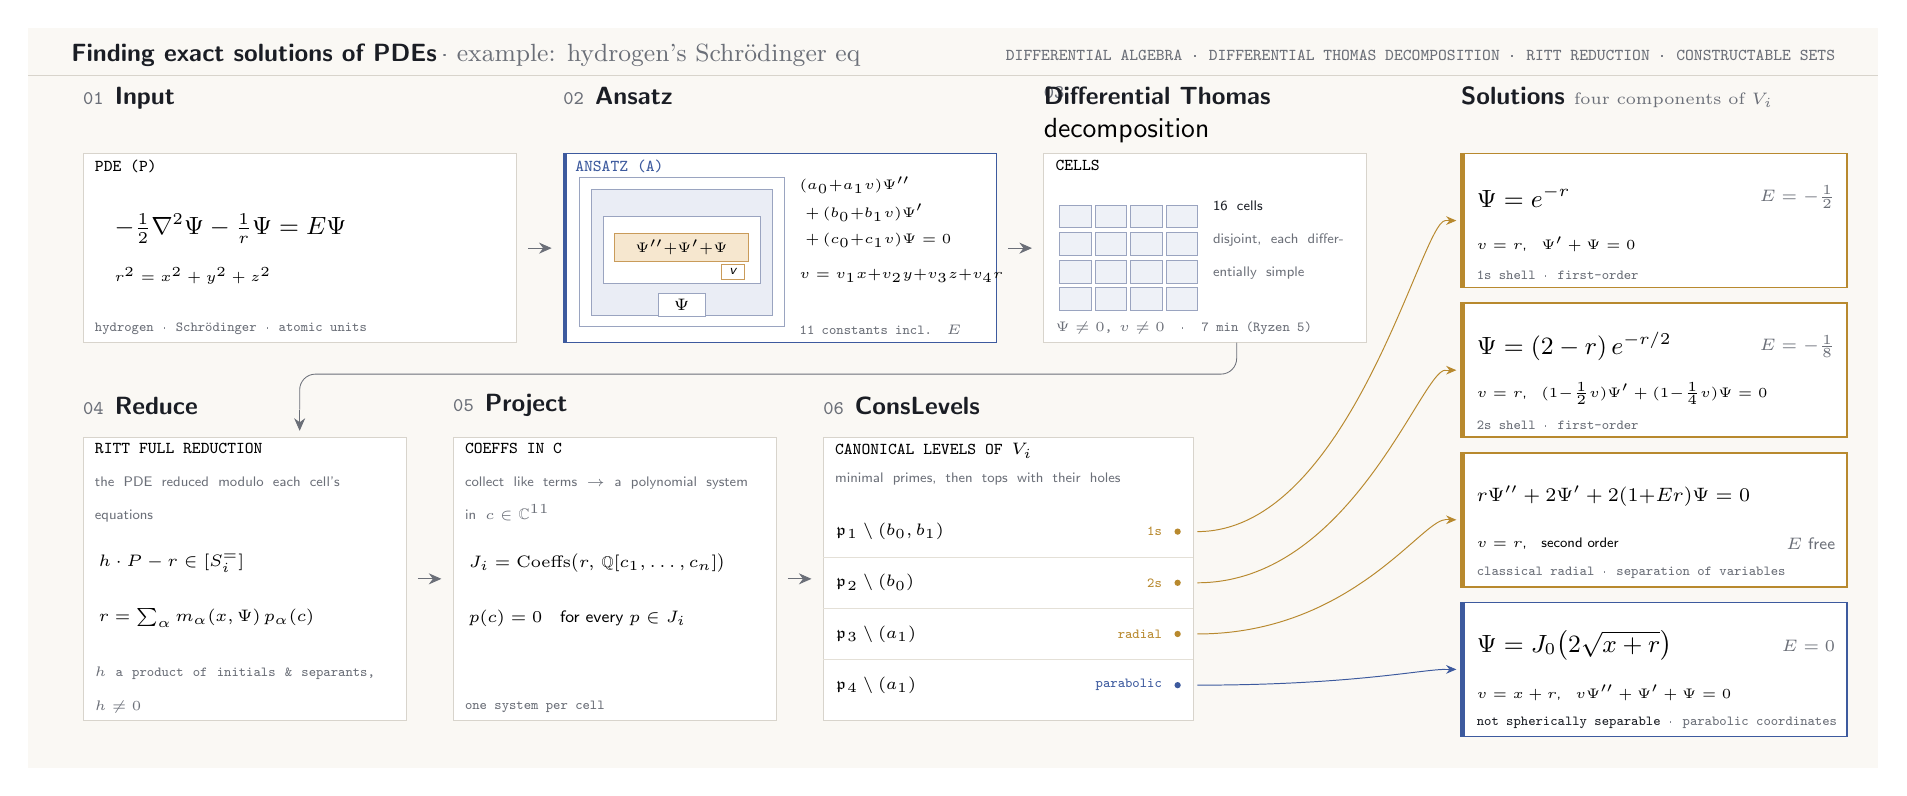
\begin{tikzpicture}[x=1mm, y=1mm, font=\sffamily]

% ========== BACKGROUND ==========
\fill[bgcol] (0,0) rectangle (235, 94);

% ========== HEADER STRIP ==========
\node[anchor=west] at (5.5, 90.5)
  {\bfseries\small\color{ink} Finding exact solutions of PDEs%
   \color{faint}\normalfont\,\textperiodcentered\ example: hydrogen's Schr\"odinger eq};
\node[anchor=east] at (229.5, 90.5)
  {\ttfamily\color{faint}\fontsize{6.5pt}{7.8pt}\selectfont
   DIFFERENTIAL ALGEBRA \textperiodcentered\ DIFFERENTIAL THOMAS DECOMPOSITION \textperiodcentered\ RITT REDUCTION \textperiodcentered\ CONSTRUCTABLE SETS};
\draw[faintrule] (0, 88) -- (235, 88);

% ==================================================================
% ROW 1 OF THE WORKFLOW — 01 Input, 02 Ansatz, 03 Decomposition
% cards y 54..78, stage heads anchored north-west at y 86.5
% ==================================================================

% ---------- 01 INPUT ----------
\node[anchor=north west] at (7, 86.5) {\stagehead{1}{Input}};
\draw[card] (7, 54) rectangle (62, 78);
\node[anchor=north west] at (8.5, 77.2) {\upper{PDE\ (P)}};
\node[anchor=west] at (11, 68.5)
  {\small$-\tfrac{1}{2}\nabla^{2}\Psi - \tfrac{1}{r}\Psi = E\Psi$};
\node[anchor=west] at (11, 62.5)
  {\fontsize{5.5pt}{6.5pt}\selectfont$r^{2} = x^{2}+y^{2}+z^{2}$};
\node[anchor=south west] at (8.5, 55)
  {\note{hydrogen \textperiodcentered\ Schr\"odinger \textperiodcentered\ atomic units}};

\draw[arrowhead] (63.5, 66) -- (66.5, 66);

% ---------- 02 ANSATZ ----------
\node[anchor=north west] at (68, 86.5) {\stagehead{2}{Ansatz}};
\draw[cardA] (68, 54) rectangle (123, 78);
\draw[accent, line width=1.2pt] (68.3, 54) -- (68.3, 78);
\node[anchor=north west] at (69.5, 77.2)
  {\ttfamily\fontsize{6.2pt}{7.5pt}\selectfont\color{accent}\bfseries ANSATZ\ (A)};

% ----- the first ansatz of \S\ref{sec:Ansatze}: one linear 2nd-order ODE -----
\begin{scope}[shift={(83, 65.5)}]
  % outer frame
  \draw[ringBorder, line width=0.3pt, fill=paper] (-13, -9.5) rectangle (13, 9.5);
  % ring background
  \fill[ringBg, draw=ringBorder, line width=0.15pt] (-11.5, -8) rectangle (11.5, 8);
  % inner ring paper
  \fill[paper, draw=ringBorder, line width=0.15pt] (-10, -4) rectangle (10, 4.5);
  % ODE strip
  \fill[odeBg, draw=odeBorder, line width=0.15pt] (-8.5, -1.2) rectangle (8.5, 2.4);
  \node at (0, 0.6) {\fontsize{4.8pt}{5.8pt}\selectfont\itshape $\Psi''{+}\Psi'{+}\Psi$};
  % v box hanging off the ODE
  \draw[odeBorder, line width=0.15pt, fill=paper] (5, -3.4) rectangle (8, -1.6);
  \node at (6.5, -2.5) {\fontsize{4.4pt}{5.2pt}\selectfont\itshape v};
  % Psi output
  \draw[ringBorder, line width=0.2pt, fill=paper] (-3, -8.2) rectangle (3, -5.2);
  \node at (0, -6.7) {\fontsize{6pt}{7pt}\selectfont\itshape$\Psi$};
\end{scope}

% ----- the ansatz as differential polynomials -----
\node[anchor=west] at (98, 74)
  {\fontsize{4.8pt}{5.8pt}\selectfont$(a_0{+}a_1 v)\Psi''$};
\node[anchor=west] at (98, 70.5)
  {\fontsize{4.8pt}{5.8pt}\selectfont$\;{+}\,(b_0{+}b_1 v)\Psi'$};
\node[anchor=west] at (98, 67)
  {\fontsize{4.8pt}{5.8pt}\selectfont$\;{+}\,(c_0{+}c_1 v)\Psi = 0$};
\node[anchor=west] at (98, 62.5)
  {\fontsize{4.6pt}{5.5pt}\selectfont$v = v_1 x{+}v_2 y{+}v_3 z{+}v_4 r$};
\node[anchor=south west] at (98, 55)
  {\note{11 constants incl. $E$}};

\draw[arrowhead] (124.5, 66) -- (127.5, 66);

% ---------- 03 DIFFERENTIAL THOMAS DECOMPOSITION ----------
% Card 03 stops at x=170 rather than 178: the fan-out below needs a clear
% corridor to climb through on its way to the topmost solution card.
% Drawn as two nodes so the second line hangs under "Differential" rather than
% under "03".  \ttfamily stays scoped to the number and the title gets
% \bfseries\small over the picture's \sffamily -- exactly as \stagehead does it.
% The line break is explicit: left to itself TeX hyphenates "de-composition".
\node[anchor=north west] at (129, 86.5)
  {\ttfamily\scriptsize\color{faint}03};
\node[anchor=north west, xshift=\stagenumwd, align=left] at (129, 86.5)
  {\bfseries\small\color{ink}Differential Thomas\\decomposition};
\draw[card] (129, 54) rectangle (170, 78);
\node[anchor=north west] at (130.5, 77.2) {\upper{cells}};

% 4 x 4 grid of cells: the decomposition's 16 differentially simple systems
\foreach \c in {0,1,2,3} {
  \foreach \rw in {0,1,2,3} {
    \draw[cellbox] ($(131, 71.5) + (\c*4.5, -\rw*3.5)$)
      rectangle ++(4.0, -2.9);
  }
}
\node[anchor=north west, text width=18mm, align=left] at (150.5, 72)
  {\fontsize{5.5pt}{7pt}\selectfont\color{ink}16 cells\\
   \color{faint}disjoint, each differentially simple};
\node[anchor=south west] at (130.5, 55)
  {\note{$\Psi \neq 0$,\ $v \neq 0$ \ \textperiodcentered\ \ 7 min (Ryzen 5)}};

% ---------- RETURN SWEEP INTO ROW 2 ----------
\draw[faint, line width=0.3pt, rounded corners=2mm]
  (153.5, 54) -- (153.5, 50) -- (34.5, 50) -- (34.5, 45.5);
\draw[arrowhead] (34.5, 45.5) -- (34.5, 42.8);

% ==================================================================
% ROW 2 OF THE WORKFLOW — 04 Reduce, 05 Project, 06 ConsLevels
% cards y 6..42, stage heads at y 46
% ==================================================================

% ---------- 04 REDUCE ----------
\node[anchor=west] at (7, 46) {\stagehead{4}{Reduce}};
\draw[card] (7, 6) rectangle (48, 42);
\node[anchor=north west] at (8.5, 41.2) {\upper{ritt full reduction}};
\node[anchor=north west, text width=37mm] at (8.5, 37)
  {\fontsize{5.5pt}{7pt}\selectfont\color{faint} the PDE reduced modulo each cell's equations};
\node[anchor=west] at (9, 26)
  {\fontsize{6.5pt}{8pt}\selectfont$h \cdot P - r \in [S^=_i]$};
\node[anchor=west] at (9, 19)
  {\fontsize{6.5pt}{8pt}\selectfont$r = \sum_\alpha m_\alpha(x,\Psi)\, p_\alpha(c)$};
\node[anchor=south west, text width=37mm, align=left] at (8.5, 7)
  {\note{$h$ a product of initials \& separants,\ $h \neq 0$}};

\draw[arrowhead] (49.5, 24) -- (52.5, 24);

% ---------- 05 PROJECT ----------
\node[anchor=west] at (54, 46) {\stagehead{5}{Project}};
\draw[card] (54, 6) rectangle (95, 42);
\node[anchor=north west] at (55.5, 41.2) {\upper{coeffs in c}};
\node[anchor=north west, text width=37mm] at (55.5, 37)
  {\fontsize{5.5pt}{7pt}\selectfont\color{faint} collect like terms $\rightarrow$ a polynomial system in $c \in \mathbb{C}^{11}$};
% Notation as in Algorithm 2; the paper reports no equation count for the
% hydrogen run, so none is claimed here.
\node[anchor=west] at (56, 26)
  {\fontsize{5.6pt}{7pt}\selectfont$J_i = \mathrm{Coeffs}\bigl(r,\, \mathbb{Q}[c_1, \ldots, c_n]\bigr)$};
\node[anchor=west] at (56, 19)
  {\fontsize{5.6pt}{7pt}\selectfont$p(c) = 0 \quad\text{for every } p \in J_i$};
\node[anchor=south west] at (55.5, 7)
  {\note{one system per cell}};

\draw[arrowhead] (96.5, 24) -- (99.5, 24);

% ---------- 06 CONSLEVELS ----------
\node[anchor=west] at (101, 46) {\stagehead{6}{ConsLevels}};
\draw[card] (101, 6) rectangle (148, 42);
\node[anchor=north west] at (102.5, 41.2) {\upper{canonical levels of $V_i$}};
\node[anchor=north west, text width=43mm] at (102.5, 37.5)
  {\fontsize{5.5pt}{7pt}\selectfont\color{faint} minimal primes, then tops with their holes};

% the four locally closed components, as computed in \S\ref{sec:Example}
\foreach \y in {26.75, 20.25, 13.75} { \draw[hairrule] (101, \y) -- (148, \y); }

\node[anchor=west] at (102.5, 30)
  {\fontsize{5.6pt}{7pt}\selectfont$\mathfrak{p}_1 \setminus (b_0, b_1)$};
\node[anchor=east] at (144, 30)
  {\ttfamily\fontsize{5.4pt}{6.6pt}\selectfont\color{amber}\bfseries 1s};
\fill[amber] (146, 30) circle (0.4);

\node[anchor=west] at (102.5, 23.5)
  {\fontsize{5.6pt}{7pt}\selectfont$\mathfrak{p}_2 \setminus (b_0)$};
\node[anchor=east] at (144, 23.5)
  {\ttfamily\fontsize{5.4pt}{6.6pt}\selectfont\color{amber}\bfseries 2s};
\fill[amber] (146, 23.5) circle (0.4);

\node[anchor=west] at (102.5, 17)
  {\fontsize{5.6pt}{7pt}\selectfont$\mathfrak{p}_3 \setminus (a_1)$};
\node[anchor=east] at (144, 17)
  {\ttfamily\fontsize{5.4pt}{6.6pt}\selectfont\color{amber}\bfseries radial};
\fill[amber] (146, 17) circle (0.4);

\node[anchor=west] at (102.5, 10.5)
  {\fontsize{5.6pt}{7pt}\selectfont$\mathfrak{p}_4 \setminus (a_1)$};
\node[anchor=east] at (144, 10.5)
  {\ttfamily\fontsize{5.4pt}{6.6pt}\selectfont\color{accent}\bfseries parabolic};
\fill[accent] (146, 10.5) circle (0.4);

% ---------- FAN-OUT FROM THE FOUR LEVELS TO THE FOUR SOLUTIONS ----------
\foreach \ys/\yb/\col in {30/69.5/amber, 23.5/50.5/amber, 17/31.5/amber, 10.5/12.5/accent} {
  \draw[\col, line width=0.35pt]
    (148.5, \ys) .. controls (168, \ys) and (177, \yb) .. (180, \yb);
  \draw[\col, line width=0.35pt, -{Stealth[length=1.3mm,width=1.1mm]}]
    (180, \yb) -- (181.4, \yb);
}

% ==================================================================
% SOLUTIONS — the four components of the intermediate locus
% cards x 182..231
% ==================================================================
\node[anchor=north west] at (182, 86.5)
  {\bfseries\small\color{ink}Solutions%
   \ \color{faint}\normalfont\fontsize{6pt}{7.2pt}\selectfont four components of $V_i$};

% ---- 1s (first-order) ----
\draw[cardAmber] (182, 61) rectangle (231, 78);
\draw[amber, line width=1.2pt] (182.3, 61) -- (182.3, 78);
\node[anchor=west] at (184, 72.5) {\small$\Psi = e^{-r}$};
\node[anchor=east] at (229.5, 72.5) {\fontsize{6.5pt}{8pt}\selectfont\color{faint}$E = -\tfrac{1}{2}$};
\node[anchor=west] at (184, 66.5)
  {\fontsize{5.2pt}{6.4pt}\selectfont$v = r$,\quad $\Psi' + \Psi = 0$};
\node[anchor=south west] at (184, 62)
  {\note{1s shell \textperiodcentered\ first-order}};

% ---- 2s (first-order) ----
\draw[cardAmber] (182, 42) rectangle (231, 59);
\draw[amber, line width=1.2pt] (182.3, 42) -- (182.3, 59);
\node[anchor=west] at (184, 53.5) {\small$\Psi = (2-r)\,e^{-r/2}$};
\node[anchor=east] at (229.5, 53.5) {\fontsize{6.5pt}{8pt}\selectfont\color{faint}$E = -\tfrac{1}{8}$};
\node[anchor=west] at (184, 47.5)
  {\fontsize{5.2pt}{6.4pt}\selectfont$v = r$,\quad $(1{-}\tfrac{1}{2}v)\Psi' + (1{-}\tfrac{1}{4}v)\Psi = 0$};
\node[anchor=south west] at (184, 43)
  {\note{2s shell \textperiodcentered\ first-order}};

% ---- generic radial (a family in E) ----
\draw[cardAmber] (182, 23) rectangle (231, 40);
\draw[amber, line width=1.2pt] (182.3, 23) -- (182.3, 40);
\node[anchor=west] at (184, 34.5)
  {\fontsize{7pt}{8.5pt}\selectfont$r\Psi'' + 2\Psi' + 2(1{+}Er)\Psi = 0$};
\node[anchor=east] at (229.5, 28.5) {\fontsize{6.5pt}{8pt}\selectfont\color{faint}$E$ free};
\node[anchor=west] at (184, 28.5)
  {\fontsize{5.2pt}{6.4pt}\selectfont$v = r$,\quad second order};
\node[anchor=south west] at (184, 24)
  {\note{classical radial \textperiodcentered\ separation of variables}};

% ---- parabolic / Bessel ----
\draw[cardA] (182, 4) rectangle (231, 21);
\draw[accent, line width=1.2pt] (182.3, 4) -- (182.3, 21);
\node[anchor=west] at (184, 15.5) {\small$\Psi = J_0\!\left(2\sqrt{x+r}\right)$};
\node[anchor=east] at (229.5, 15.5) {\fontsize{6.5pt}{8pt}\selectfont\color{faint}$E = 0$};
\node[anchor=west] at (184, 9.5)
  {\fontsize{5.2pt}{6.4pt}\selectfont$v = x + r$,\quad $v\Psi'' + \Psi' + \Psi = 0$};
\node[anchor=south west] at (184, 5)
  {\fontsize{5.5pt}{6.8pt}\selectfont\ttfamily\color{ink}not spherically separable%
   \ \color{faint}\textperiodcentered\ parabolic coordinates};

\end{tikzpicture}
\end{document}
